\chapter*{Simulering af indgangsvælger}

Følgende simuleringer er foretaget ved 200 mV @ 1 kHz som indgangssignal. Der er foretaget en AC sweep, en FFT og en THD analyse for følgende situationer: MIC tændt, LINE tændt og begge tændt. Bemærk at der er indgangssignal på begge kanaler under målingerne således at bidraget fra den dæmpede kanal kommer med i THD målingen. Følgende kredsløb er simuleret:

\begin{figure}[h]
\centering
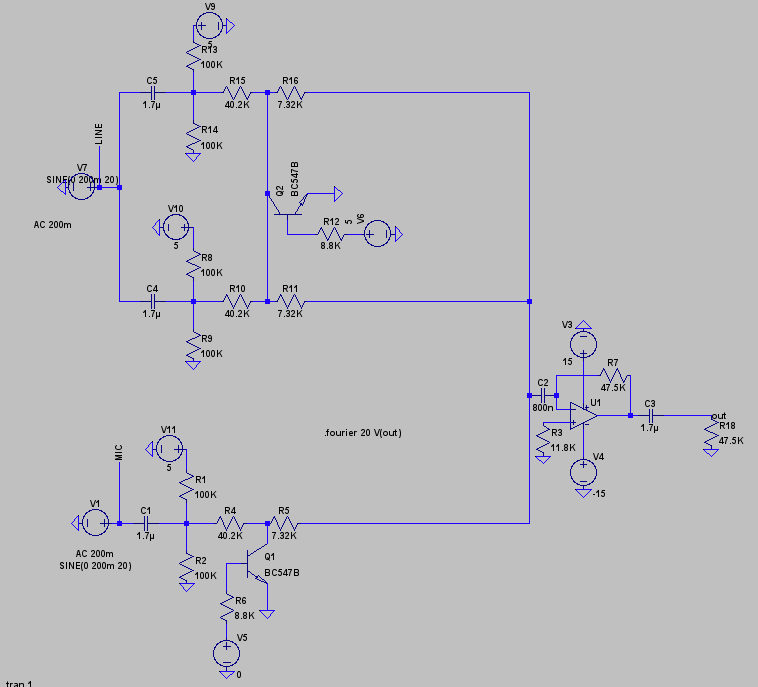
\includegraphics[scale=.6]{/implementering/indgangsvaelger/simulering/indgangsvaelger-circuit.png}
\caption{Indgangsvælgerens kredsløbsdesign}
\label{}
\end{figure}


\section*{MIC tændt}
Total Harmonic Distortion: 0.016746\%



\section*{LINE tændt}
Total Harmonic Distortion: 0.025662\%


\section*{Både MIC og LINE tændt}
Total Harmonic Distortion: 0.016991%






